%=================================================================
\section{Introduction}
\label{sec-intro}
   (1)Bike-sharing is not new to us. This report mainly analyzes the data of bike-sharing in Washington, US from 2011 to 2012.\\
   (2) The data comes from Kaggle https://www.kaggle.com/c/bike-sharing-demand.\\
   (3) This project is mainly about the prediction of relevant data, and the description and analysis of relevant factors are presented here.\\
   (4) Related elements: datetime  season  holiday  workingday  weather temp  atemp 
   humidity  windspeed  casual  registered  count 
\section{Data Analysis} \label{sec-preliminaries}

First of all, our work can be divided into the following steps:\\
(1)   Descriptive statistics of the data
\begin{center}
  \begin{minipage}{1\linewidth}
  \centering
  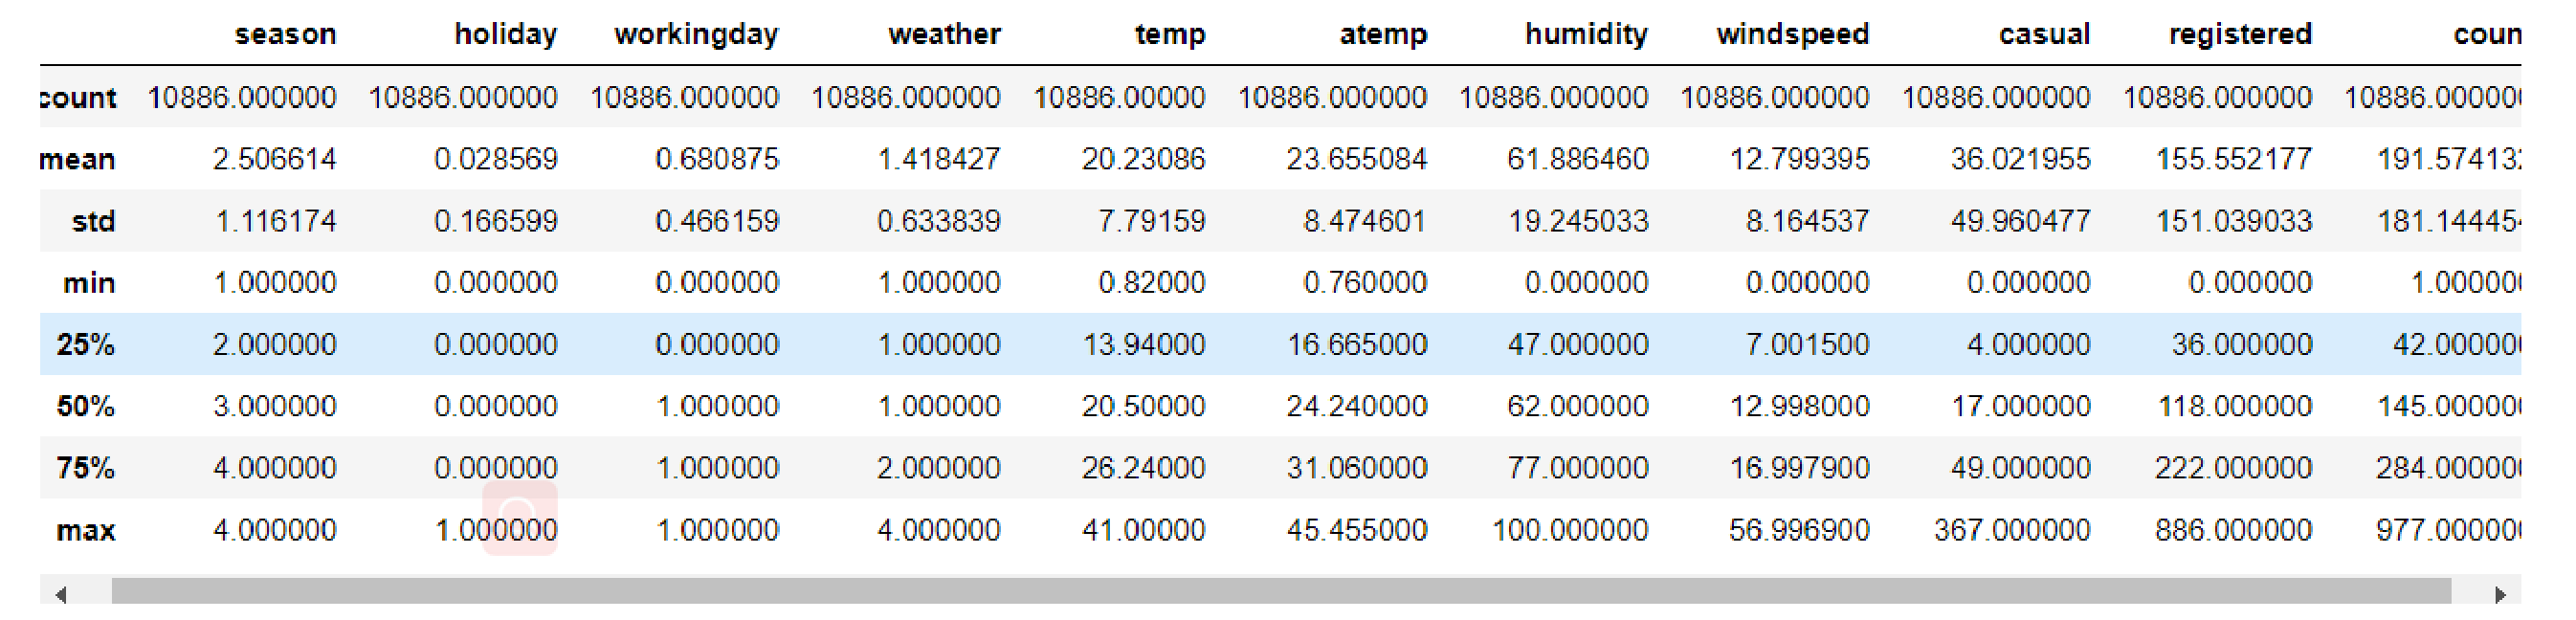
\includegraphics[width=0.6\textwidth]{pic/a.eps}
  \end{minipage}
  \hfill
\end{center}

(2) The standard deviation of the number of leases you have to predict at the end is very large.So let's look at the distribution by drawing it.\\
\begin{center}
  \begin{minipage}{0.5\linewidth}
  \centering
  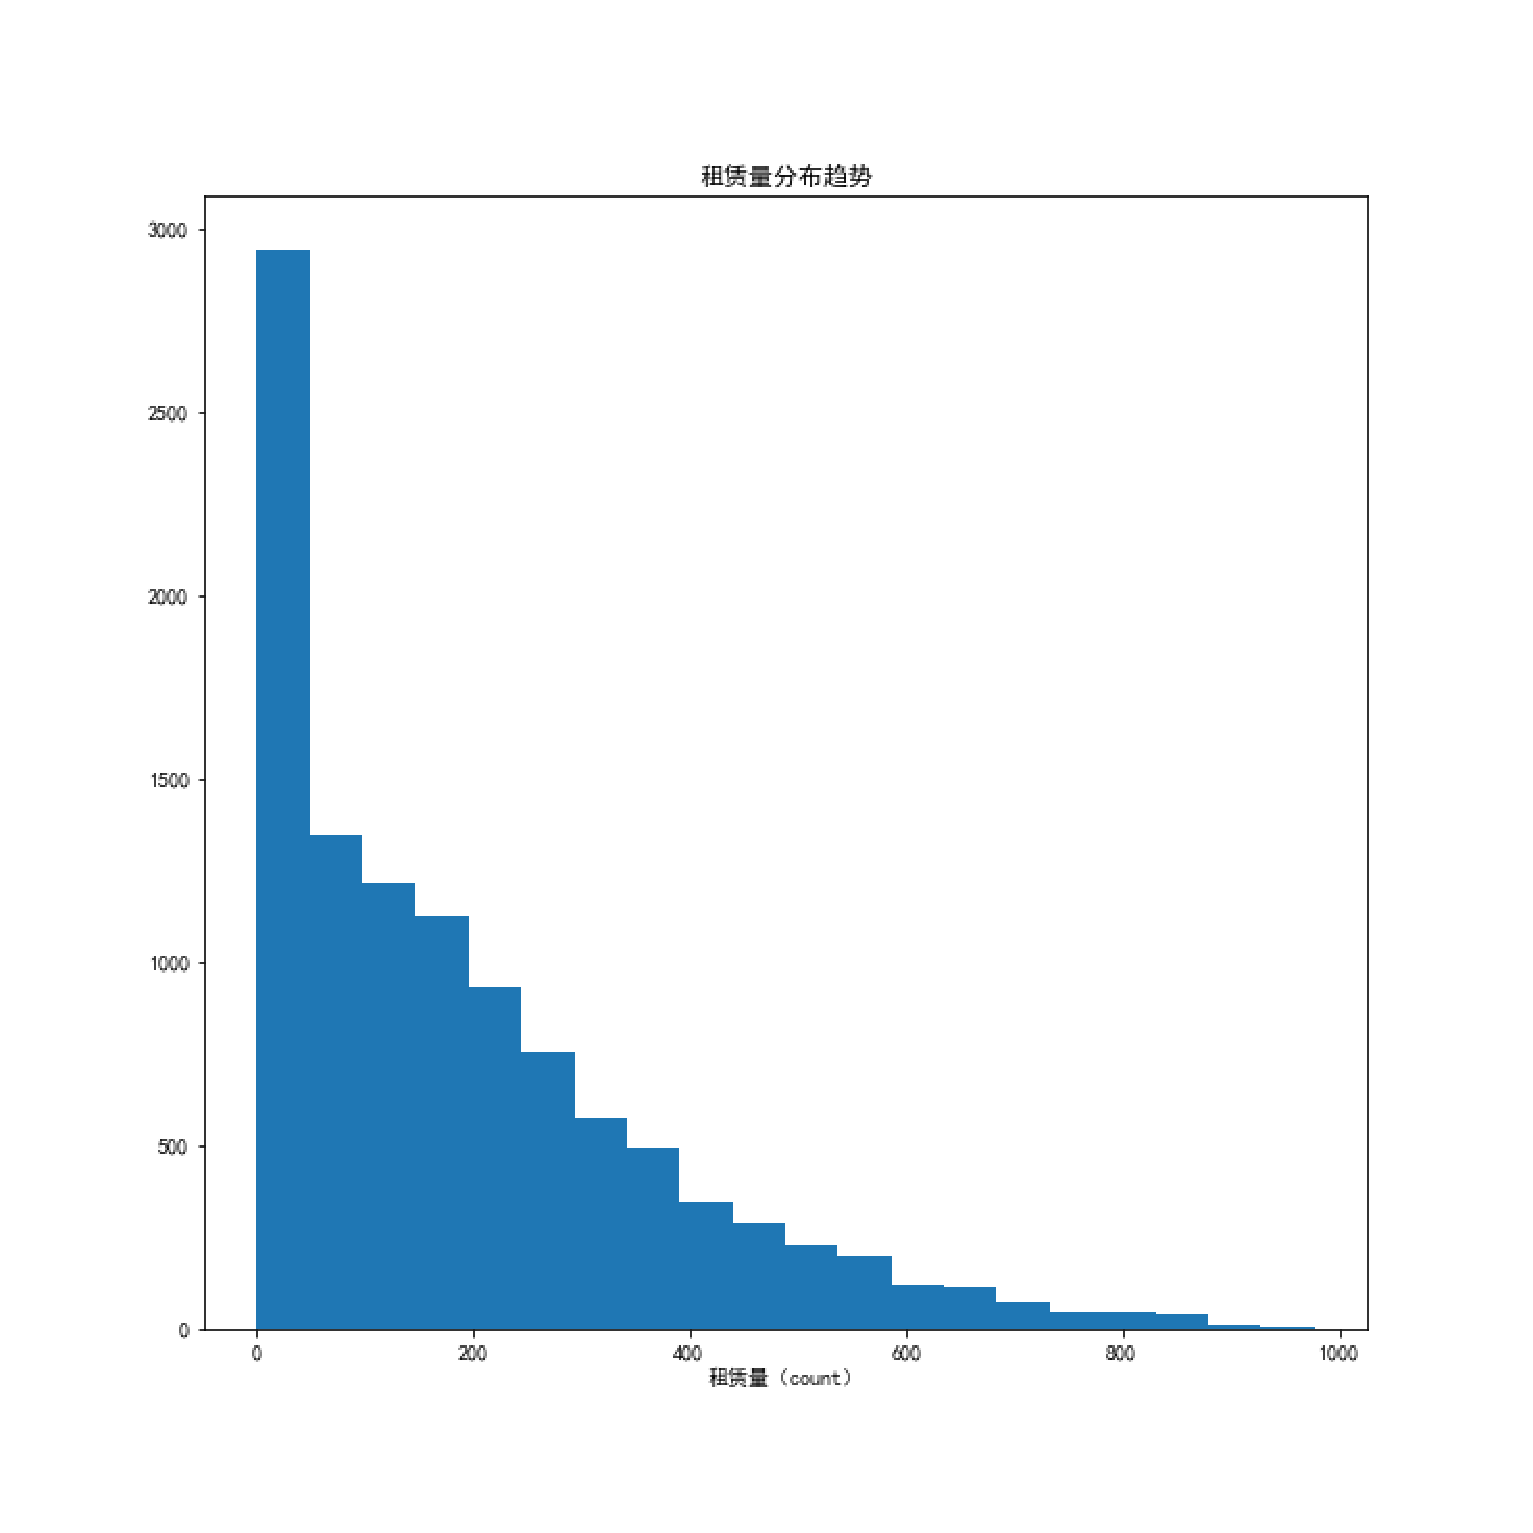
\includegraphics[width=0.55\textwidth]{pic/count .eps}
\end{minipage}

  \hfill
\end{center}
(3) Exclude data other than three standards,log of count
\begin{center}
  \begin{minipage}{1\linewidth}
    \centering
    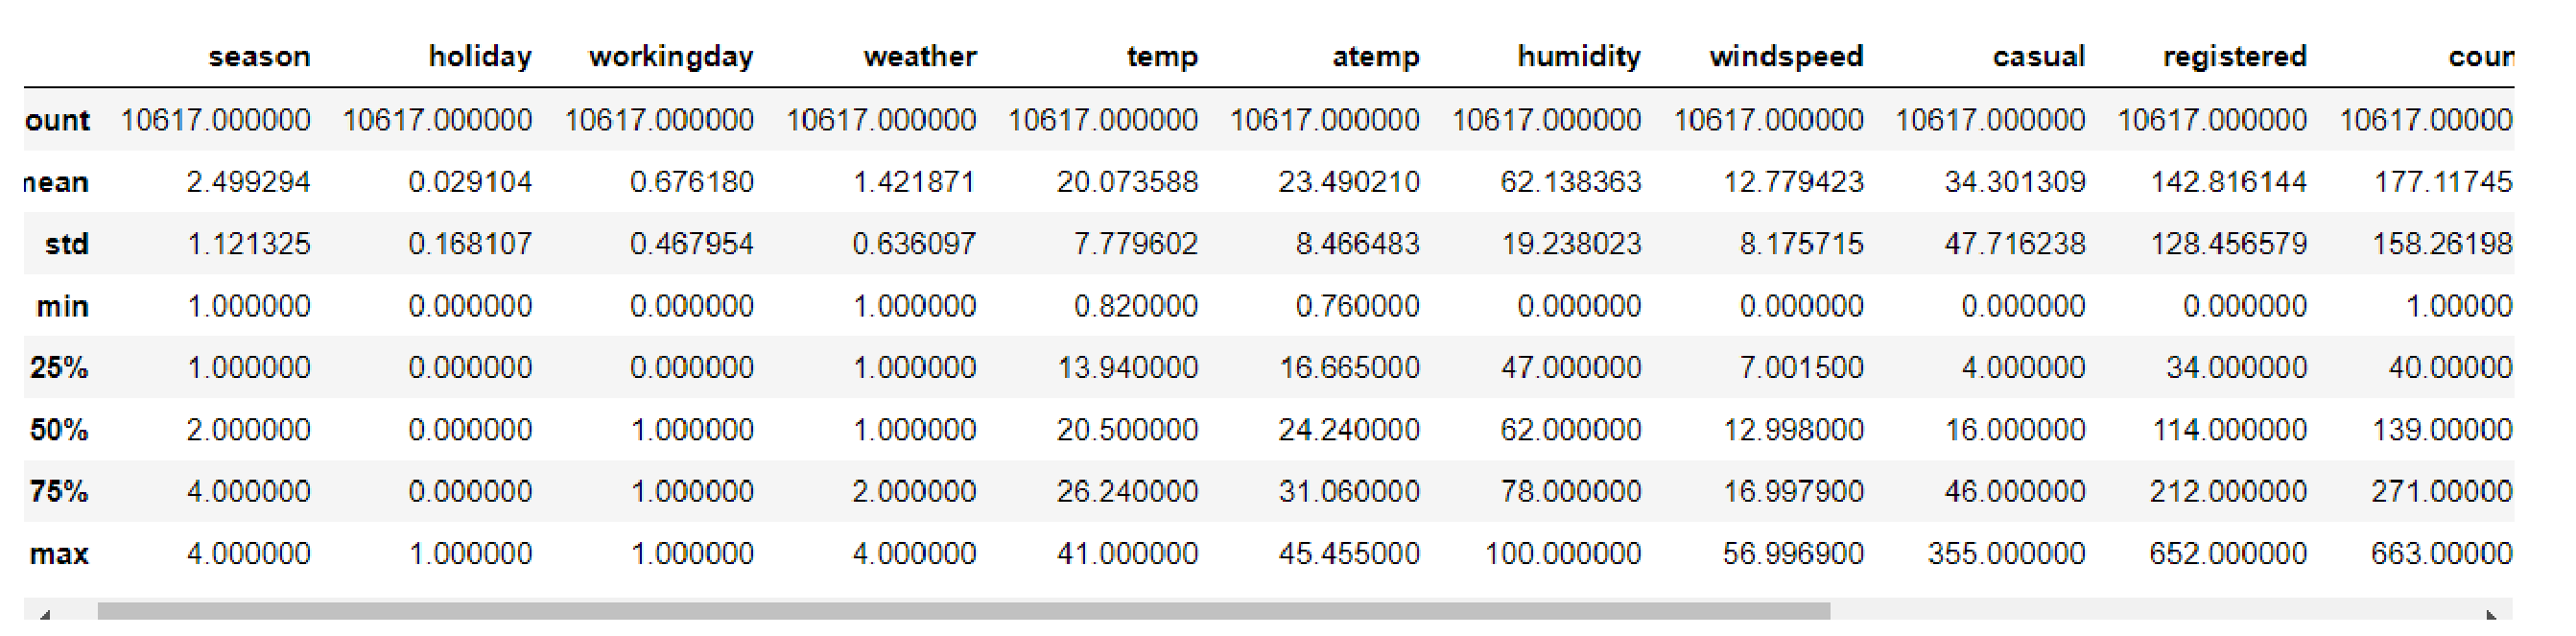
\includegraphics[width=0.7\textwidth]{pic/b.eps}
  \end{minipage}
  
  \begin{minipage}{0.4\linewidth}
    \centering
    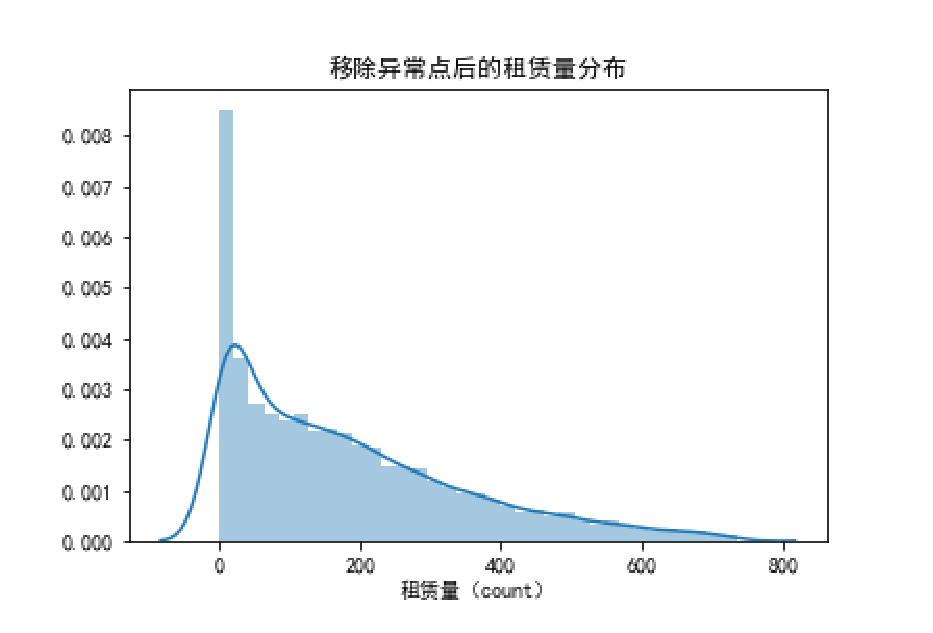
\includegraphics[height=0.7\textwidth]{pic/count a.eps}
  \end{minipage}
  
  \begin{minipage}{0.4\linewidth}
    \centering
      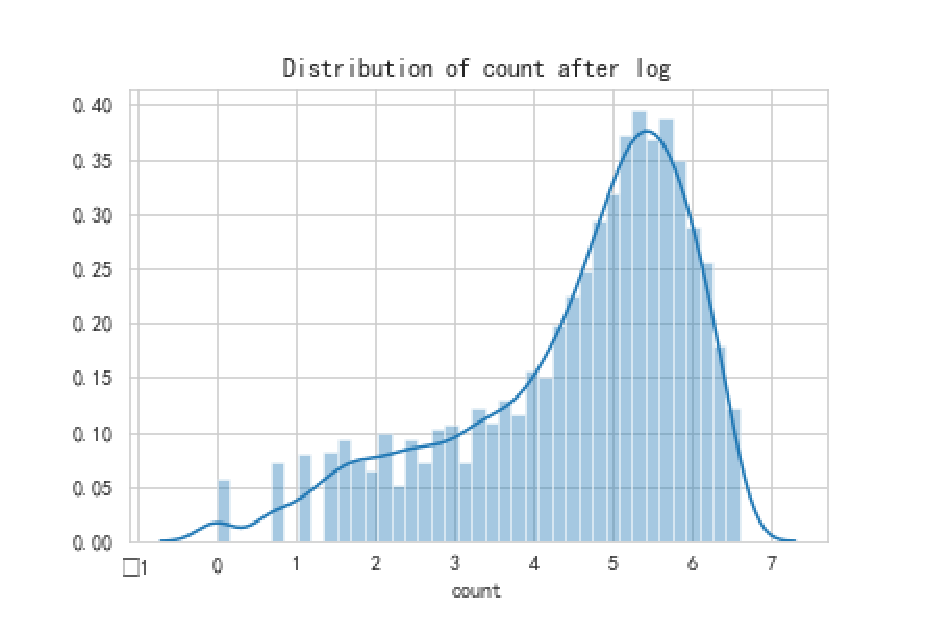
\includegraphics[height=0.7\textwidth]{pic/log.eps}
  \end{minipage}
  \hfill
\end{center}

(4)  The impact of hour,month,season,year,weekday,workingday
\begin{center}
  \begin{minipage}{0.5\linewidth}
    \centering
    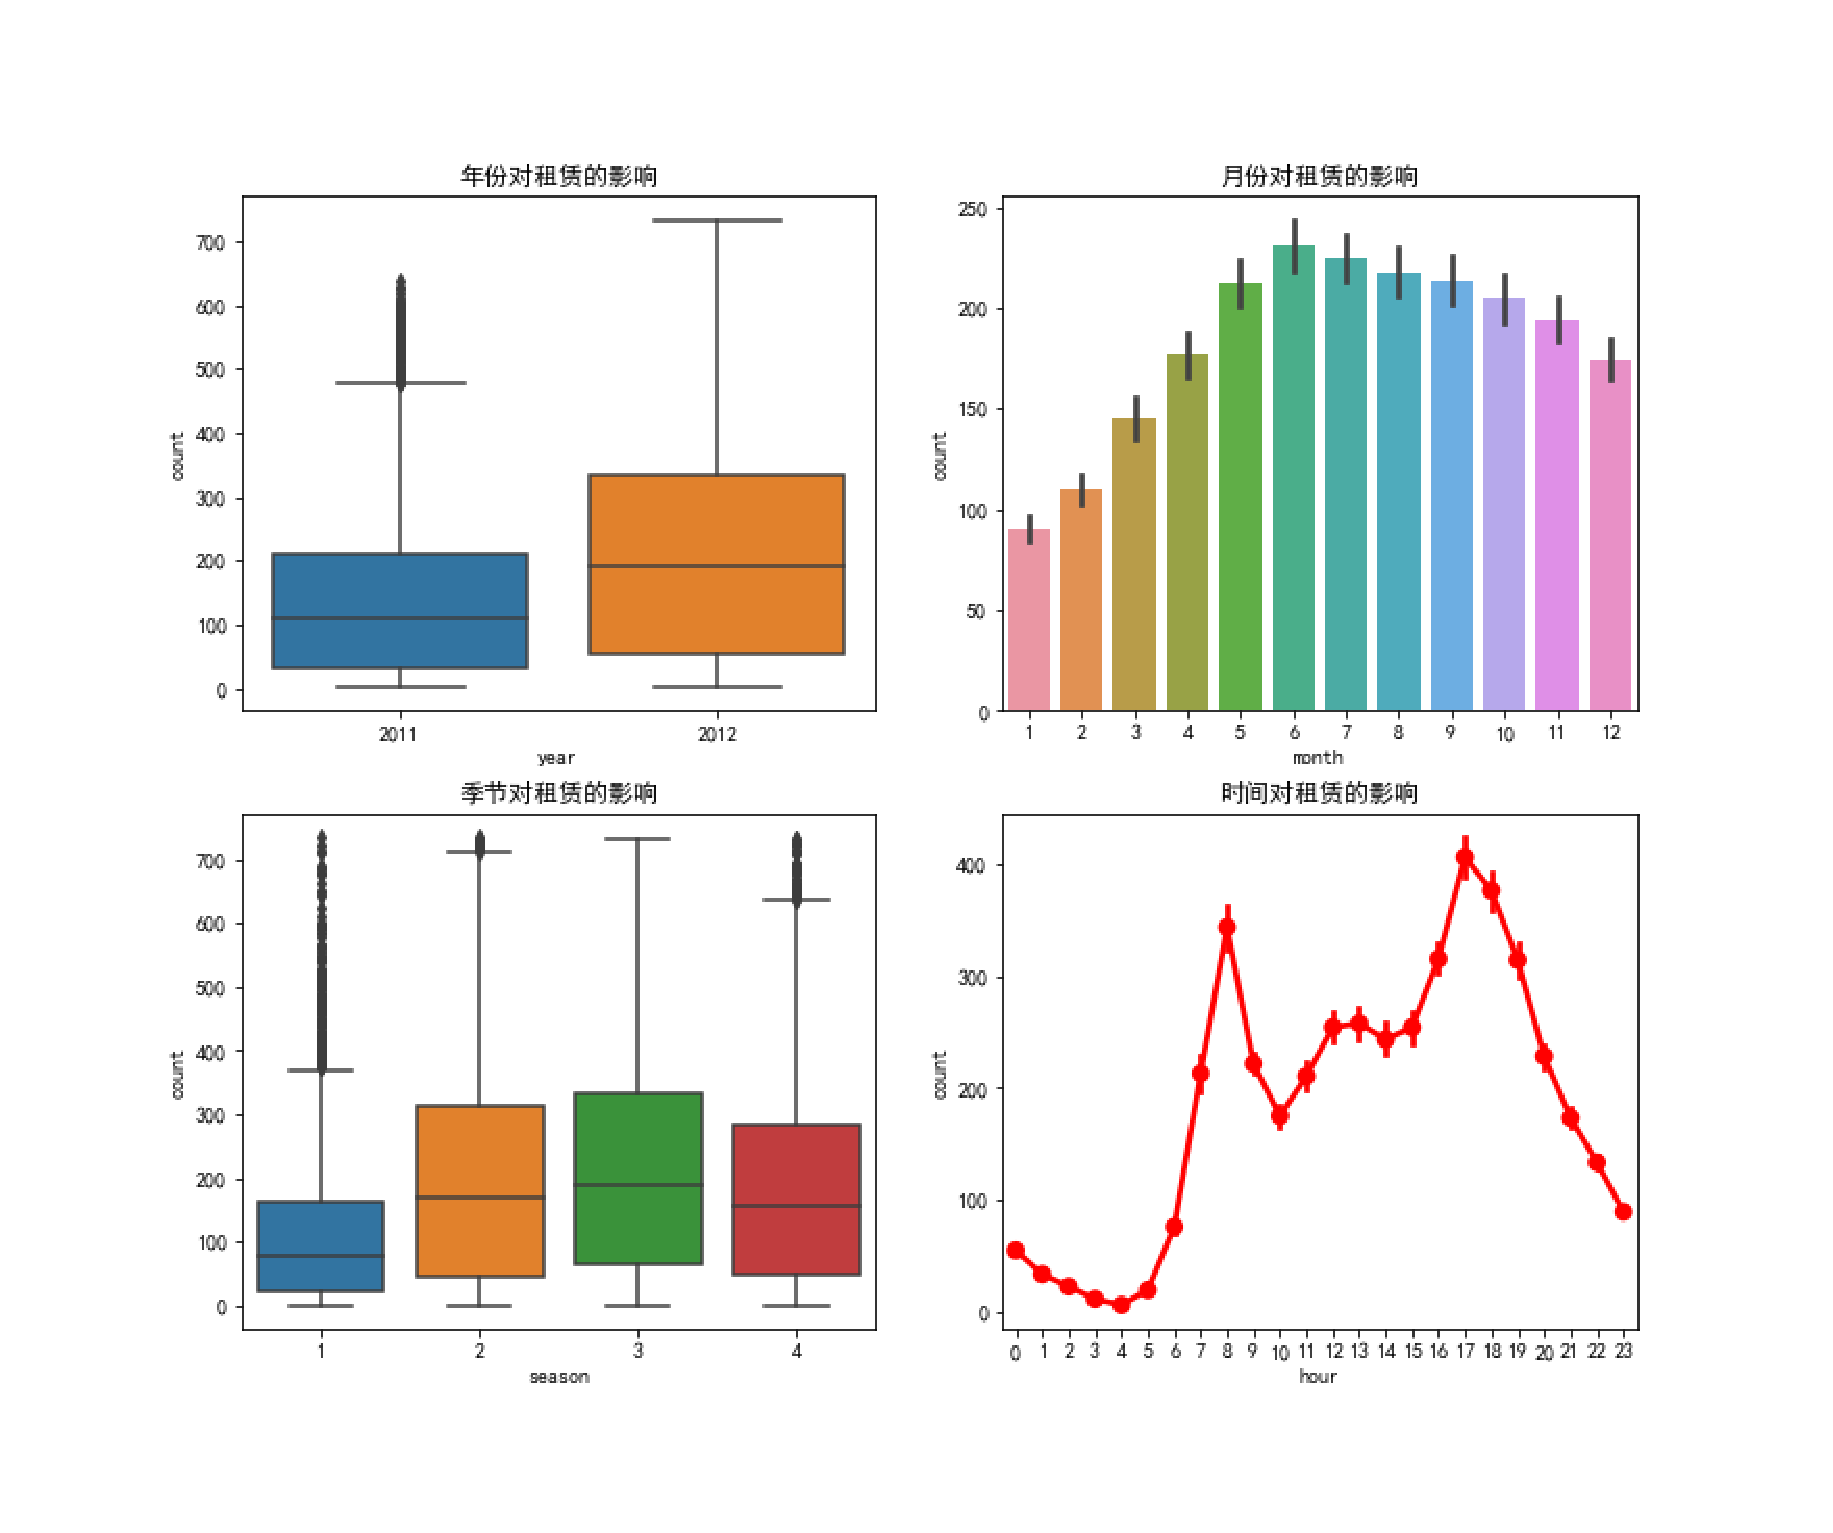
\includegraphics[height=0.8\textwidth]{pic/count all.eps}
  \end{minipage}
  
  \hfill
\end{center}




(5) The impact of temp,atemp,humidity,windspeed
\begin{center}
  \begin{minipage}[t]{1\linewidth}
    \centering
    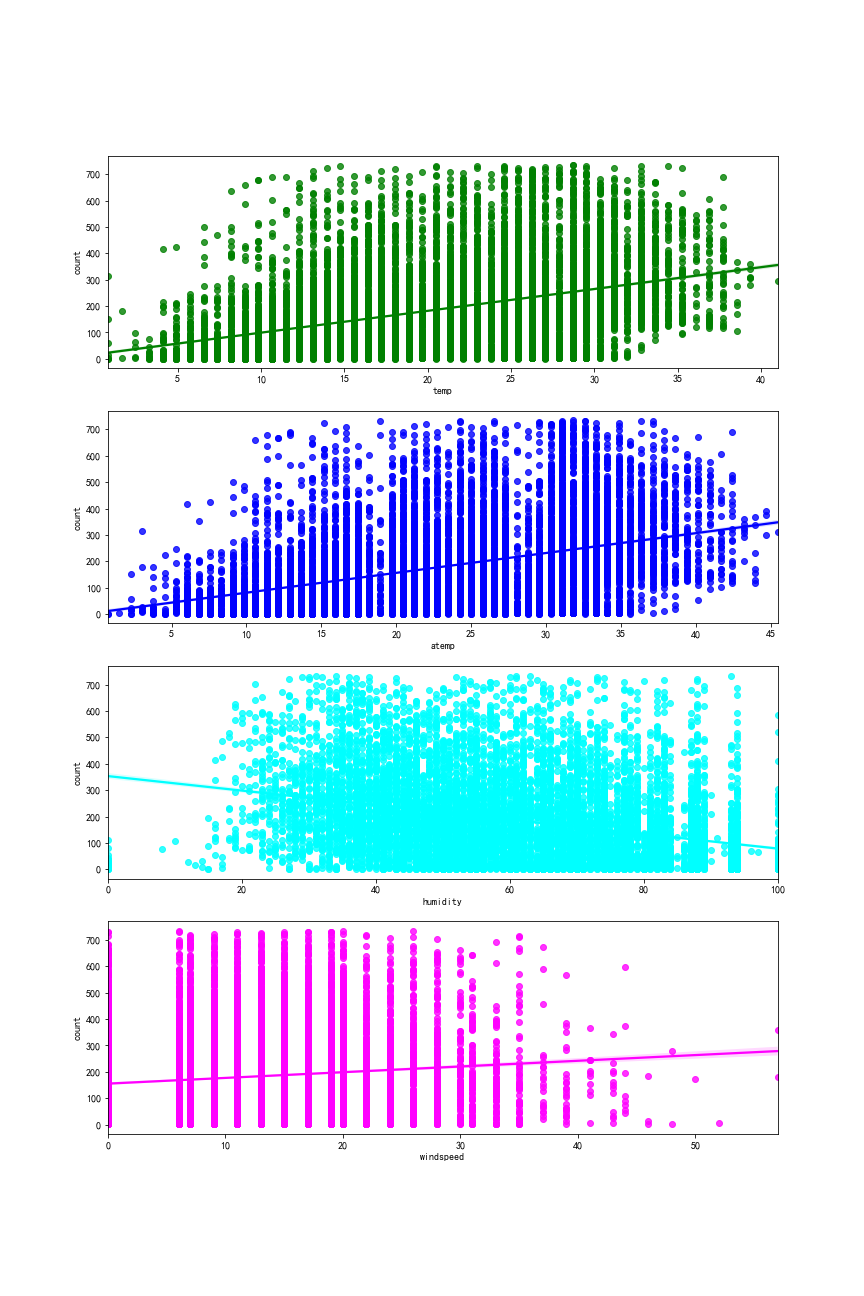
\includegraphics[width=0.5\textwidth]{pic/three tahw.png}
  \end{minipage}
  \hfill
\end{center}

(6)  The impact of weather

\begin{center}
  \begin{minipage}{0.7\linewidth}
    \centering
    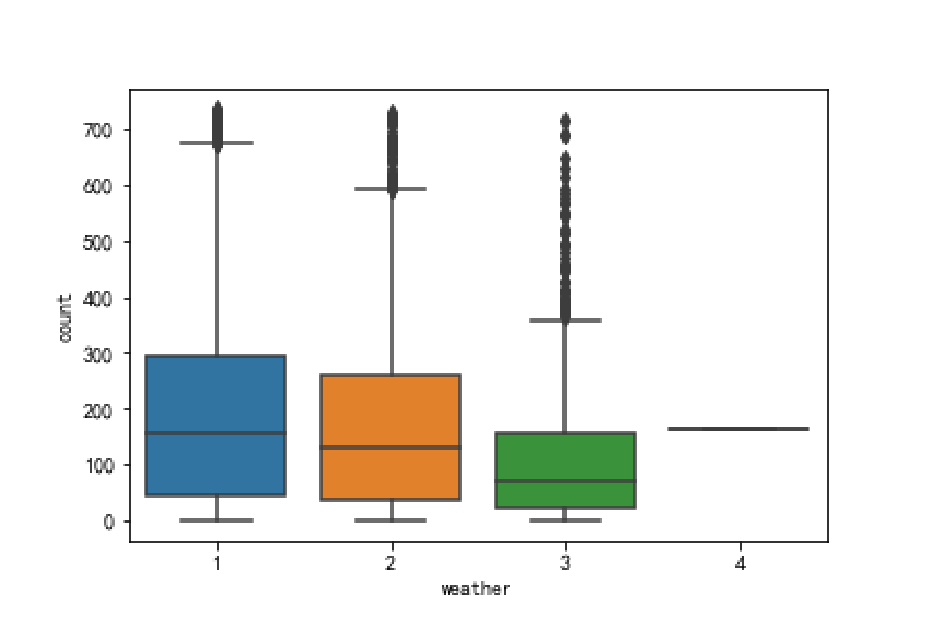
\includegraphics[height=0.7\textwidth]{pic/weather.eps}
  \end{minipage}
  \hfill
\end{center}

(7) Impact of season,week,registered and non-registered users on cycling usage trends\\
    a.For different times of the day, there is a clear trend in the use of Shared bikes, with two distinct peaks, in line with people's understanding of morning peak and evening peak.The trends were the same for all four seasons, except that usage in spring was slightly lower than in the other three.
\begin{center}
  \begin{minipage}{1\linewidth}
    \centering
    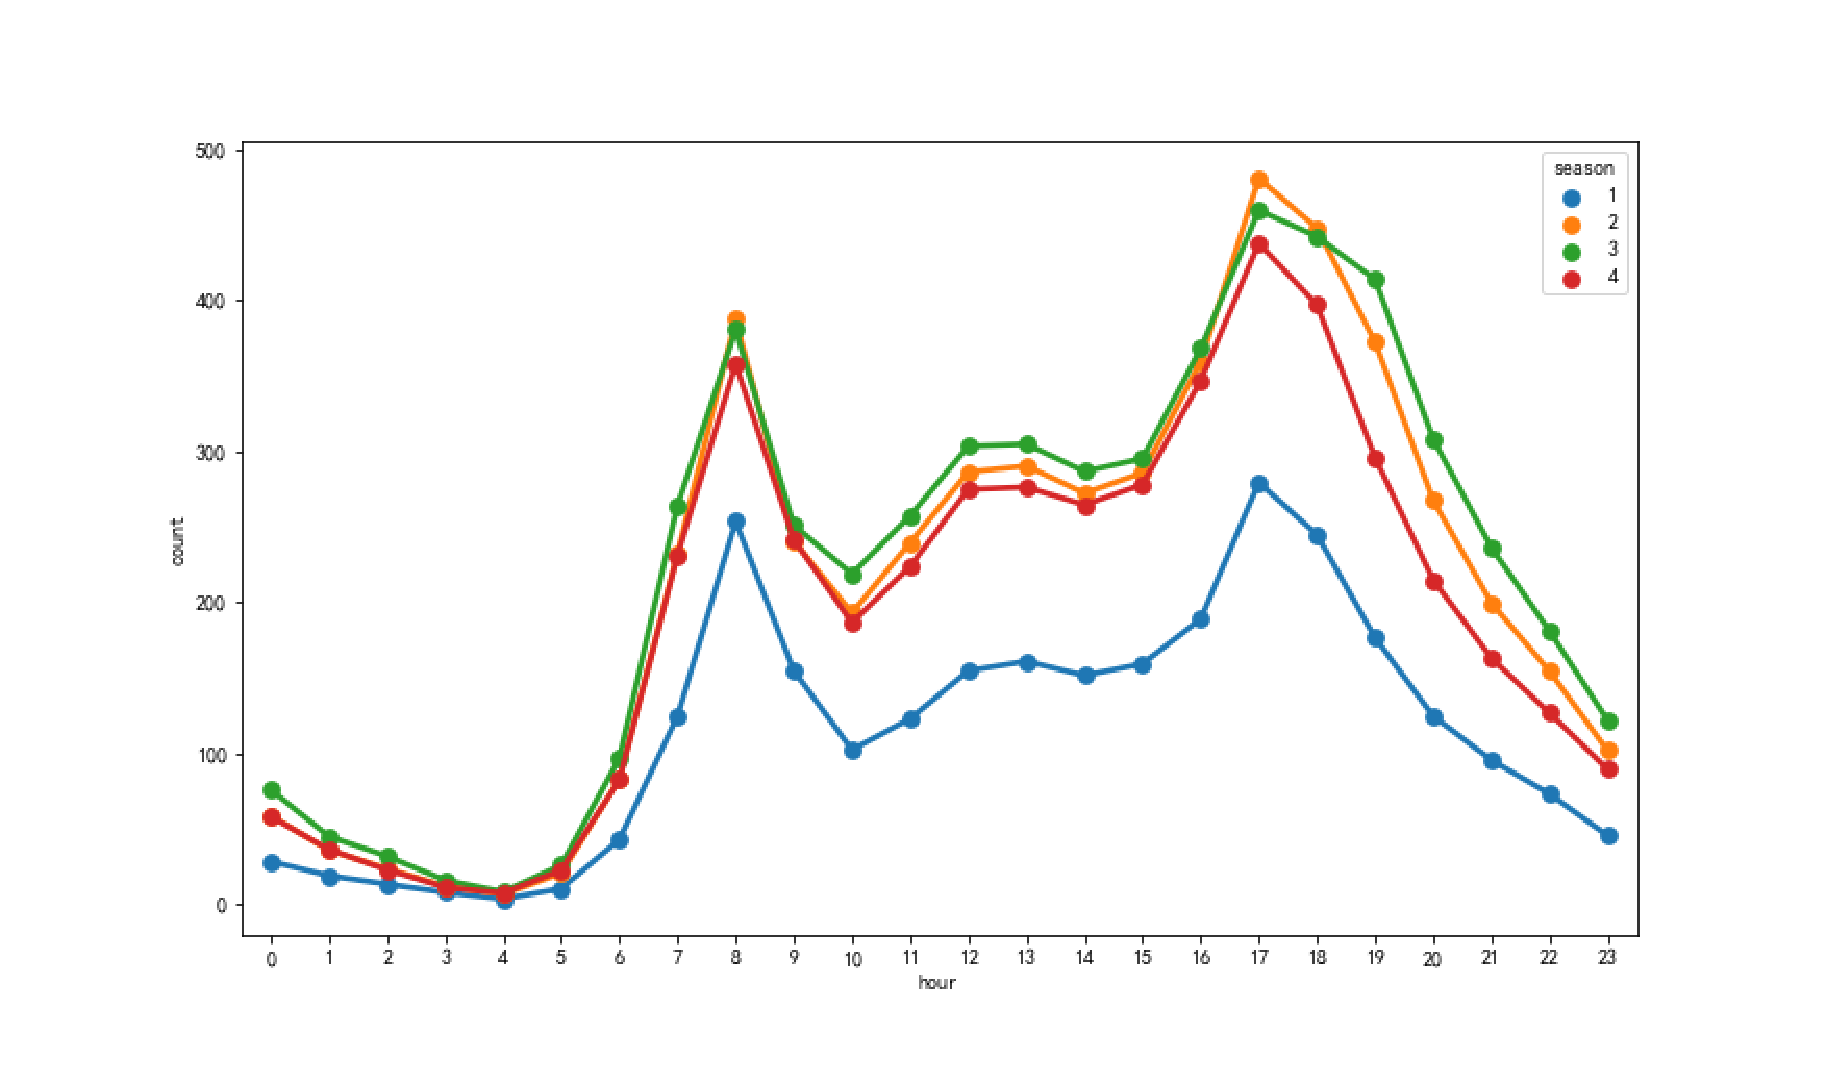
\includegraphics[width=0.7\textwidth]{pic/three hour1 (2).eps}
  \end{minipage}
  
  
  \hfill
\end{center}
b.The usage of registered users accounts for the majority of the total usage, and the trend is consistent with the total usage trend, rather than that of registered users. The usage at different times of the day does not change much, and the trend is similar to the usage trend at weekends.
\begin{center}
  \begin{minipage}{1\linewidth}
    \centering
    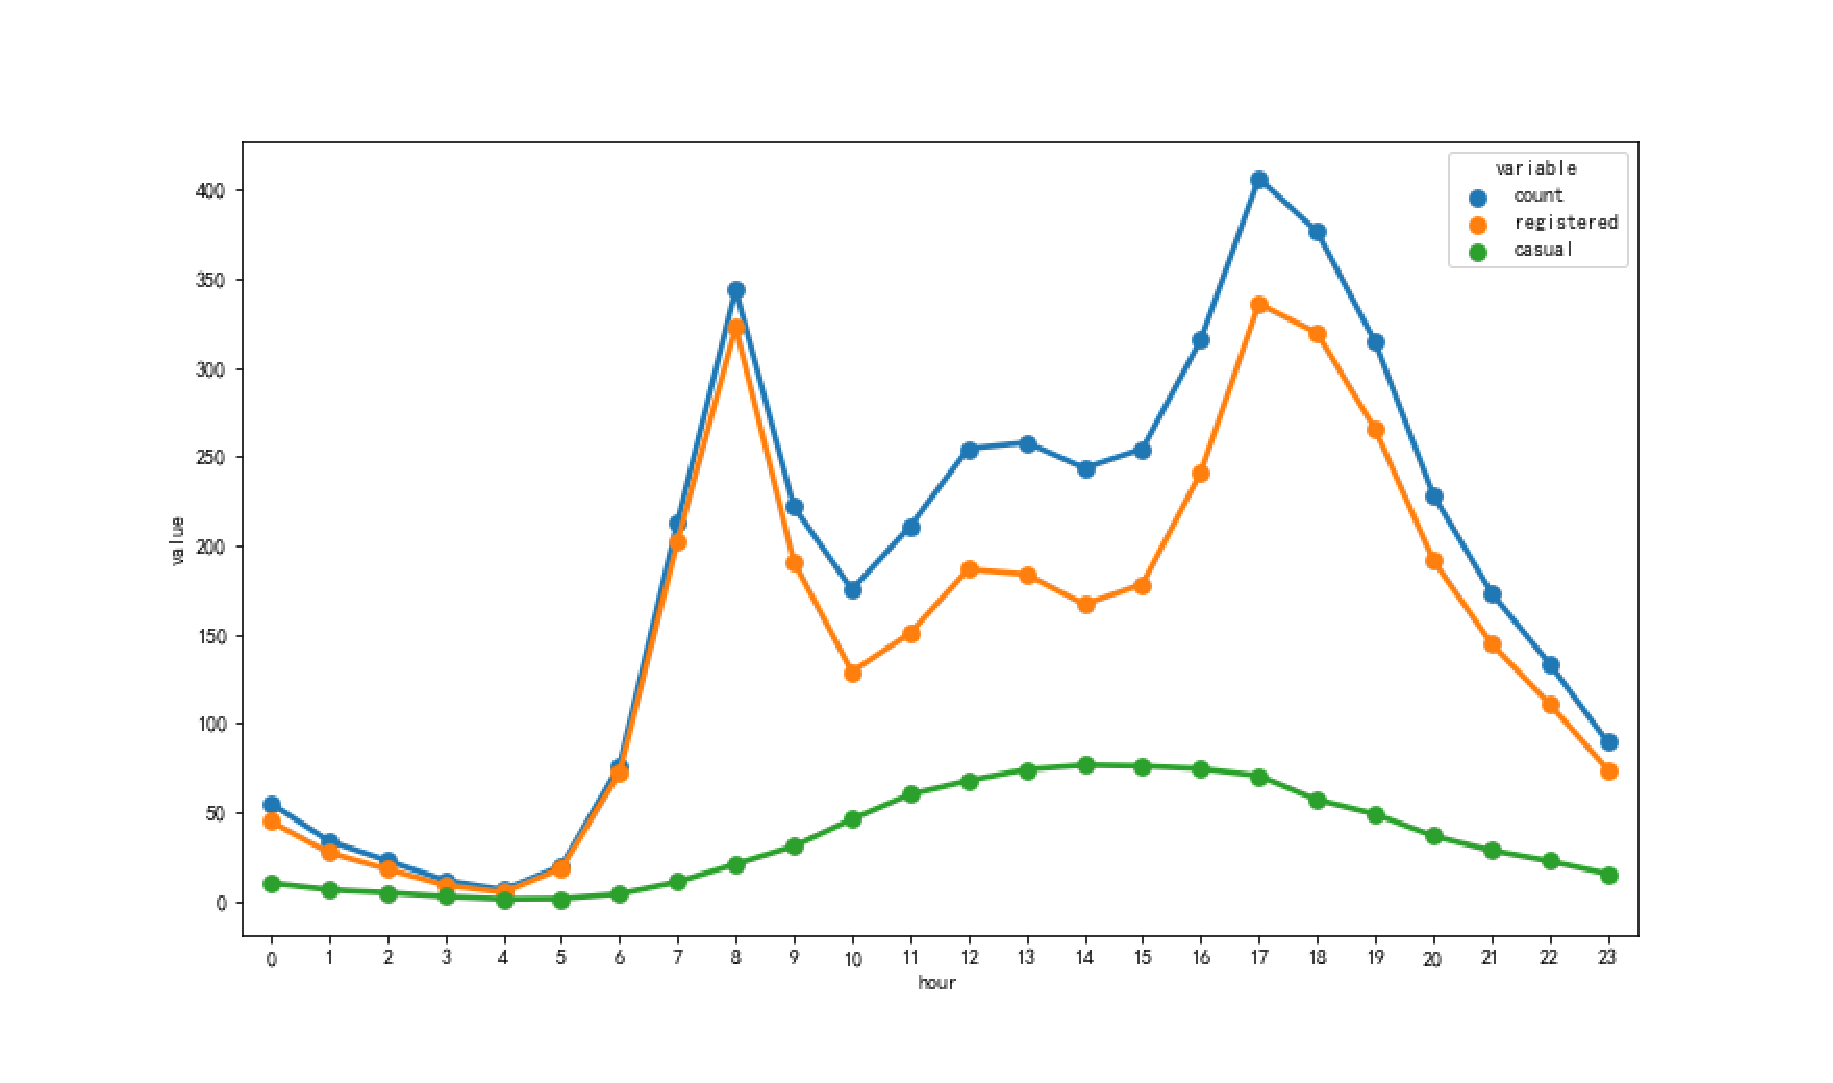
\includegraphics[width=0.7\textwidth]{pic/three hour3.eps}
  \end{minipage}
  \hfill
\end{center}
 
c.From Monday to Friday, there are two peak usage periods, while on weekends, the usage trend is completely different from that on weekdays. The usage trend changes from bimodal to flat unimodal, and the peak usage period is concentrated at 11-17 o 'clock.
\begin{center}
  \begin{minipage}{1\linewidth}
    \centering
    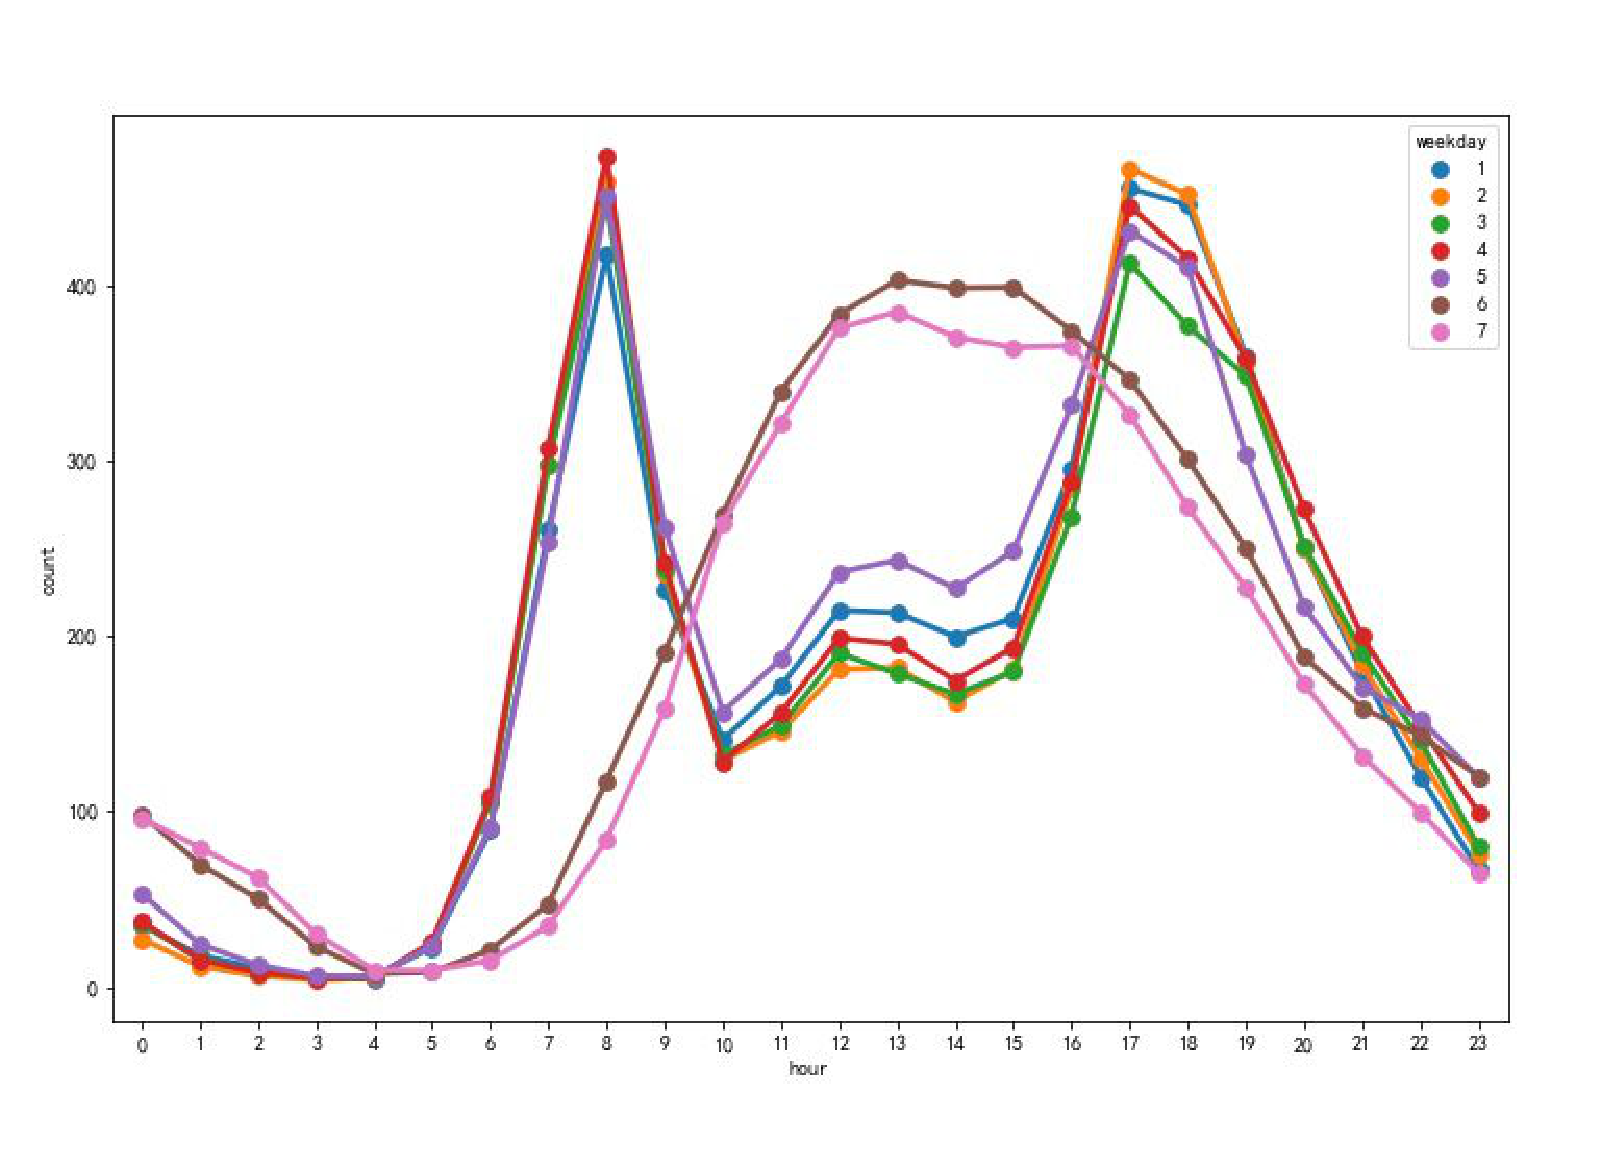
\includegraphics[width=0.7\textwidth]{pic/three hour2 (1).eps}
  \end{minipage}
  \hfill
\end{center}
 
(8)  Draw the thermal diagram of the correlation coefficient

\begin{center}
  \begin{minipage}{1\linewidth}
    \centering
    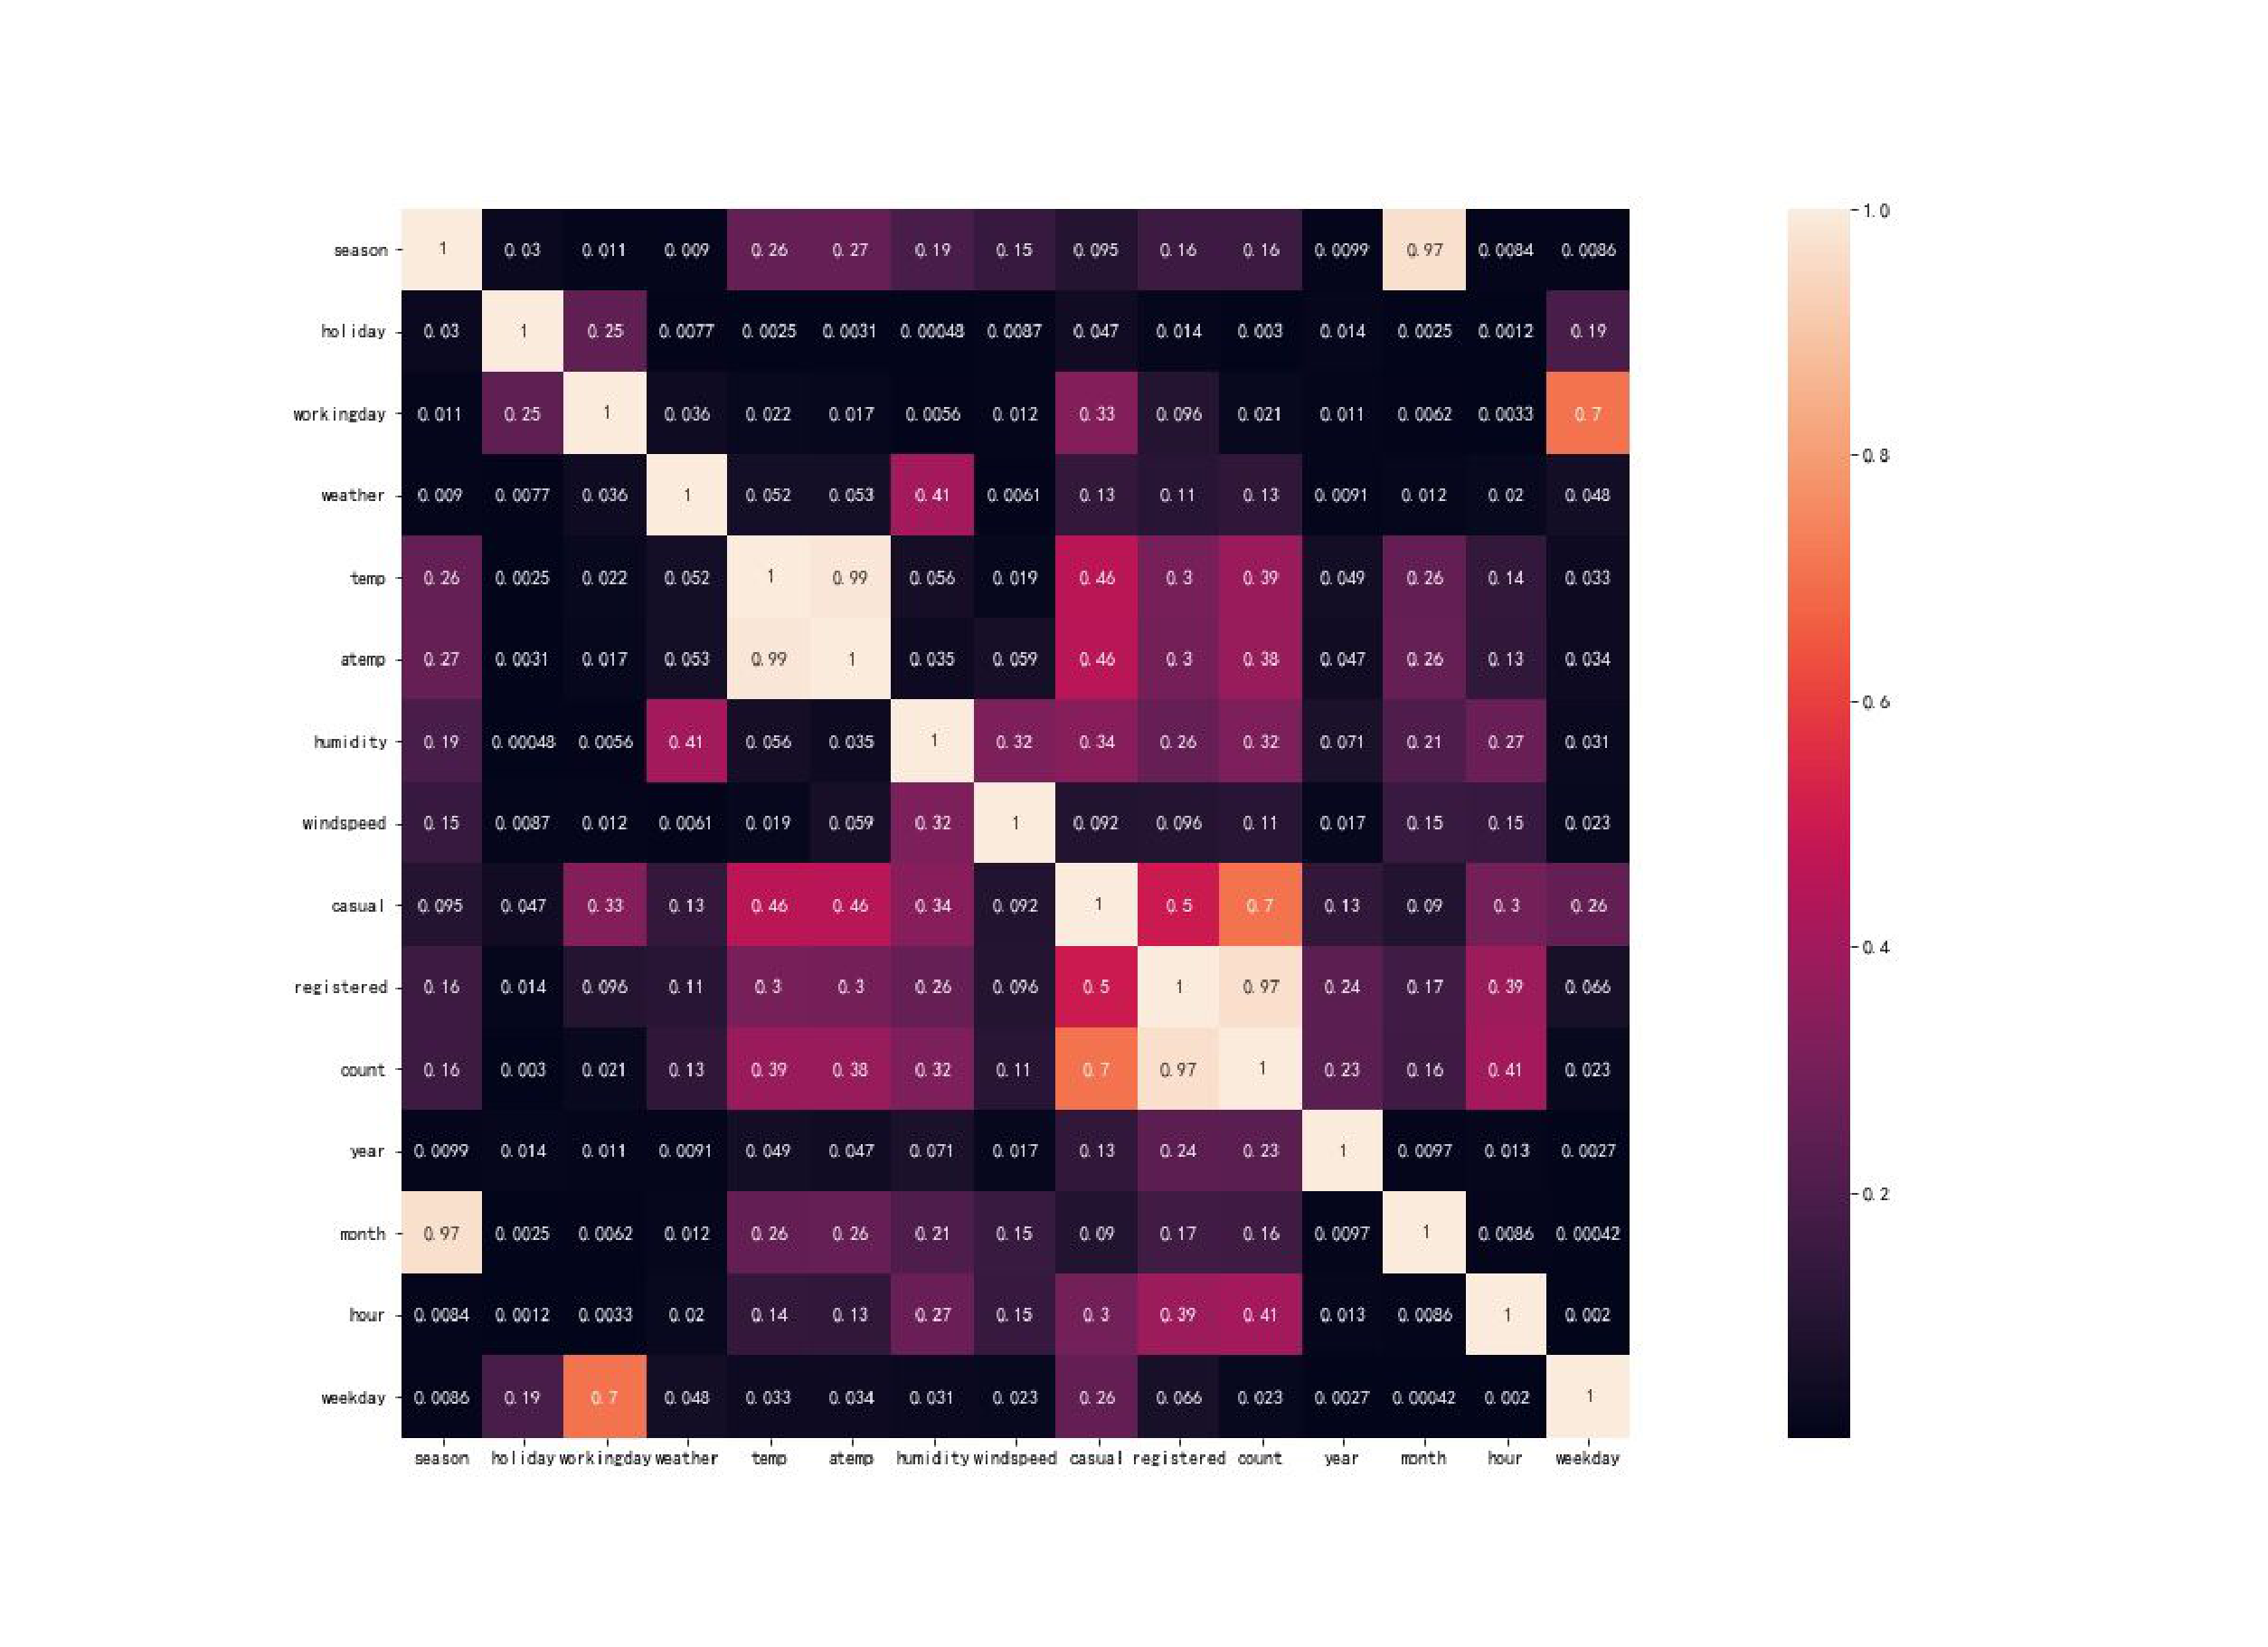
\includegraphics[height=0.5\textwidth]{pic/hot (1).eps}
  \end{minipage}
  \hfill
\end{center}


\begin{center}

  \begin{minipage}{0.3\linewidth}
  \centering

 % \includegraphics[width=0.9\textwidth]{logos/1 (3).eps}
  
  {\small{cost}}

  \end{minipage}
\end{center}
\section{Conclusions}

Through this Kaggle project, I practiced by myself to have a deeper understanding of data visualization and to explore the structure and rules of data by means of drawing and tabulating.
